\documentclass[]{article}
\usepackage{amsmath,amssymb}
\usepackage{lmodern}
\usepackage{iftex}
\usepackage{ragged2e}
\usepackage{stackengine}
\usepackage{dirtytalk}
\usepackage{graphicx}
\graphicspath{{./Images/}}
\usepackage{array}   % for \newcolumntype macro
\newcolumntype{L}{>{$}l<{$}}
\hbadness=99999

\date{May 2023}
\author{ID: 1747}
\title{Cryptology Packet Ch 6}

\begin{document}

\maketitle

\begin{enumerate}
    \item Use the Euclidean Algorithm to find the greatest common divisor for each of the following pairs of integers without using a computer.
    \begin{enumerate}
        \item $51,89$
        \\\\ $89 = 1*51+38$
        \\$51=1*38+13$
        \\$38=2*13+12$
        \\$13=1*12+1$
        \\$12=12*1+0$
        \\Therefore, the gcd(51,89)=1. 
        \item $102,202$
        \\\\ $202=1*102+100$
        \\$102=1*100+2$
        \\$100=50*2+0$
        \\Therefore, the gcd(102,202)=2.
        \item $666,1414$
        \\\\ $1414=2*666+82$
        \\$666=8*82+10$
        \\$82=8*10+2$
        \\$10=5*2+0$
        \\Therefore, the gcd(666,1414)=2.
    \end{enumerate}
    \item Use the Extended Euclidean Algorithm to express the greatest common divisor of each of the following pairs of integers as a linear combination of these integers.
    \begin{enumerate}
        \item $51,89$
        \\\\ $1=13-1(12)$
        \\$=13-1(38-2*13)$
        \\$=3(13)-1(38)$
        \\$=3(51-38)-1(38)$
        \\$=3(51)-4(38)$
        \\$=3(51)-4(89-51)$
        \\$=7(51)-4(89)$
        \\\\From the above, we have found that $x=7,y=-4$
        \item $102,202$
        \\\\ $2=102-1(100)$
        \\$=102-1(202-102)$
        \\$=2(102)-1(202)$
        \\\\From the above, we have found that $x=2,y=-1$
        \item $666,1414$
        \\\\$2=82-8(10)$
        \\$=82-8(666-8*82)$
        \\$=65(82)-8(666)$
        \\$=65(1414-2*666)-8(666)$
        \\$=65(1414)-138(666)$
        \\\\From the above, we have found that $x=65,y=-138$.
    \end{enumerate}
    \item Find $50^{-1} \mod 127$ without using a computer.
    \\\\$50x + 127y = 1$
    \\\\Using the Euclidean Algorithm:
    \\$127=2*50+27$
    \\$50=1*27+23$
    \\$27=1*23+4$
    \\$23=5*4+3$
    \\$4=1*3+1$
    \\\\Using the extended Euclidean Algorithm:
    \\$1=4-1(3)$
    \\$=4-1(23-5*4)$
    \\$=6(4)-1(23)$
    \\$=6(27-23)-1(23)$
    \\$=6(27)-7(23)$
    \\$=6(27)-7(50-27)$
    \\$=13(27)-7(50)$
    \\$=13(127-2*50)-7(50)$
    \\$=13(127)-33(50)$
    \\\\Therefore, since $127(13)+50(-33)=1$, we also know that $-33 \equiv 50^{-1} \mod 127$ and $13 \equiv 127^{-1} \mod 50$.
    \item In the RSA cryptosystem, find $D$ given $p=13,q=17$, and $E=5$
    \\\\$D=E^{-1} \mod (p-1)(q-1)$
    \\$D=5^{-1} \mod 192$
    \\\\$5x+192=1$
    \\\\Using the Euclidean Algorithm:
    \\$192=38*5+2$
    \\$5=2*2+1$
    \\\\Using the extended Euclidean Algorithm:
    \\$1=5-2(2)$
    \\$=5-2(192-5*38)$
    \\$=77(5)-2(192)$
    \\\\Therefore, since $77(5)+-2(192)=1$, we also know that $77 \equiv 5^{-1} \mod 204$. Thus, $D=77$.
    \item Write a Python function that uses the Euclidean Algorithm to find and return the greatest common divisor of two positive integers. Use your function to find the greatest common divisor for each of the following pairs of integers.
    \\\\Using a recursive algorithm for each part, we can find the greatest common divisor much quicker than by hand or a different algorithm:
    \begin{center}
        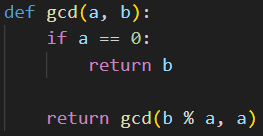
\includegraphics[scale=0.5]{EuclidAlgo.png}
    \end{center}
    \begin{enumerate}
        \item $9876543210, 123456789$
        \\\\gcd(9876543210, 123456789)=9
        \item $11111111111, 1000000001$
        \\\\gcd(11111111111, 1000000001)=1
        \item $45666020043321, 73433510078091009$
        \\\\gcd(45666020043321, 73433510078091009)=3
    \end{enumerate}

    \item Write a Python function that uses the Extended Euclidean Algorithm to write the greatest common divisor of each of the following pairs of positive integers as a linear combination of those integers.
    \\\\Using a recursive algorithm similar to the one used in the basic Euclidean Algorithm but finding $x$ and $y$ where $ax+by=gcd(a,b)$:
    \begin{center}
        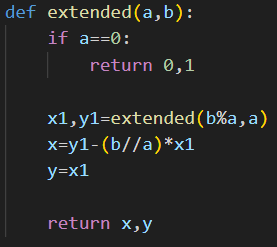
\includegraphics[scale=0.5]{Images/ExtendedEuclid.png}
    \end{center}
    \begin{enumerate}
        \item $9876543210, 123456789$
        \\\\$x=-1371742,y=109739361$
        \item $11111111111, 1000000001$
        \\\\$x=99009901,y=-1100110010$
        \item $45666020043321, 73433510078091009$
        \\\\$x=10445427205865236,y=-6495686882417$
    \end{enumerate}
    
    \item In the previous section, we used the Extended Euclidean Algorithm to find that $34 \equiv 20^{-1} \mod 97$
    \begin{enumerate}
        \item Find $20^{-1} \mod 97$ by making clever use of Euler's Theorem.
        \\\\$34 \equiv 20^{-1} \mod 97$
        \\\\Since gcd(20,97)=1, then $20^{\phi(97)} \equiv 1 \mod 97$
        \\\\$20^{\phi(97)} \equiv 1 \mod 97$
        \\$20^{96} \equiv 1 \mod 97$
        \\$20^{(96-1)} \equiv 20^{-1} \mod 97$
        \\$20^{95} \equiv 20^{-1} \mod 97$
        \\$20*(20^2)*(20^2*20^2)*(20^4*20^4)*(20^8*20^8)*(20^{16}*20^{16})*(20^{32}) \equiv 20^{-1} \mod 97$
        \\$(20*12*47*75*96*1*1) \equiv 20^{-1} \mod 97$
        \\$81216000 \equiv 20^{-1} \mod 97$
        \\$34 \equiv 20^{-1} \mod 97$
        \item Explain why using Euler's Theorem is a much more computationally difficult strategy than using the Extended Euclidean Algorithm.
        \\\\Euler’s Theorem requires calculating phi or the totient function for a given n. If n is a large number, then calculating the integers to n that are coprime involve finding prime factors of n. As n becomes larger, factoring it becomes time consuming and computationally difficult. 
        \\\\On the other hand, the Extended Euclidean Algorithm is a great tool for finding GCD and then the coefficients using Bezout’s function. Compared to Euler’s Theorem, basic calculations like multiplication, addition and subtraction can be used instead of factorization. Once we find the x and y, it also provides an efficient way of calculating modular inverses which is very important in Cryptography.
    \end{enumerate}

    
\end{enumerate}


\end{document}
